
%(BEGIN_QUESTION)
% Copyright 2008, Tony R. Kuphaldt, released under the Creative Commons Attribution License (v 1.0)
% This means you may do almost anything with this work of mine, so long as you give me proper credit

Suppose a control valve with a linear inherent characteristic and a maximum flow capacity of 18 ($C_v$ = 18) is installed at the base of a dam, where it experiences a constant upstream pressure of 20 PSI and a constant downstream pressure of 0 PSI (atmospheric):

$$\includegraphics[width=15.5cm]{i03227x01.eps}$$

Superimpose the ``load line'' for this control valve on its characteristic curve set, and then use the intersection points between the load line and the curves to determine the actual water flow rates at 0\% open, 25\% open, 50\% open, 75\% open, and 100\% (full) open:

$$\includegraphics[width=15.5cm]{i03227x02.eps}$$

$$\vbox{\offinterlineskip
\halign{\strut
\vrule \quad\hfil # \ \hfil & 
\vrule \quad\hfil # \ \hfil & 
\vrule \quad\hfil # \ \hfil \vrule \cr
\noalign{\hrule}
%
% First row
Opening & $C_v$ & Flow rate \cr
%
(\%) &  & (GPM) \cr
%
\noalign{\hrule}
%
% Another row
0 & 0 & \cr
%
\noalign{\hrule}
%
% Another row
25 & 4.5 & \cr
%
\noalign{\hrule}
%
% Another row
50 & 9 & \cr
%
\noalign{\hrule}
%
% Another row
75 & 13.5 & \cr
%
\noalign{\hrule}
%
% Another row
100 & 18 & \cr
%
\noalign{\hrule}
} % End of \halign 
}$$ % End of \vbox

\underbar{file i03227}
%(END_QUESTION)





%(BEGIN_ANSWER)

$$\includegraphics[width=15.5cm]{i03227x03.eps}$$

$$\vbox{\offinterlineskip
\halign{\strut
\vrule \quad\hfil # \ \hfil & 
\vrule \quad\hfil # \ \hfil & 
\vrule \quad\hfil # \ \hfil \vrule \cr
\noalign{\hrule}
%
% First row
Opening & $C_v$ & Flow rate \cr
%
(\%) &  & (GPM) \cr
%
\noalign{\hrule}
%
% Another row
0 & 0 & 0 \cr
%
\noalign{\hrule}
%
% Another row
25 & 4.5 & 20.1 \cr
%
\noalign{\hrule}
%
% Another row
50 & 9 & 40.2 \cr
%
\noalign{\hrule}
%
% Another row
75 & 13.5 & 60.4 \cr
%
\noalign{\hrule}
%
% Another row
100 & 18 & 80.5 \cr
%
\noalign{\hrule}
} % End of \halign 
}$$ % End of \vbox

\vskip 10pt

Follow-up question: if we were to plot a graph of flow rate ($Q$) versus valve stem opening (\%), would it be linear for this system?  Explain why or why not.

%(END_ANSWER)





%(BEGIN_NOTES)

A graph of $Q$-versus-\% opening would be quite linear, because the control valve's inherent characteristic is linear, and the pressure drop across the valve is constant.

%INDEX% Electronics review: load lines
%INDEX% Final Control Elements, valve: characterization

%(END_NOTES)


